\section{Versuchsdurchführung}
\label{sec:durchführung}
Im Folgenden werden die verschieden Messungen und deren Ergebnisse
dargestellt.
Während der gesamten Zeit musste penibel auf die Justage des Versuches
geachtet werden, denn schon eine leichte Last auf den Versuchstisch
verursachte schwankungen in der Laserleistung.

Für die Auswertung der Messergebnisse wird \texttt{python} und für die
Fehlerrechnung das Paket \texttt{uncertainties} genutzt.

\subsection{Justage}
\label{subsec:justage}
Um die Laserbedingungen zu erfüllen müssen zunächst Plasmaröhre und Spiegel der Apparatur justiert werden.
Hierfür wird -- wie in \cite{V61} beschrieben -- ein Justagelaser zur Hilfe genommen.
Der Justagelaser wird zentral auf die Plasmaröhre ausgerichtet und diese mit Hilfe eines Fadenkreuzes am Ende der optischen Schiene so eingestellt, dass der Strahl die Röhre zentral verlässt.
Anschließend wird der plane Auskopplungsspiegel direkt hinter die Plasmaröhre gestellt und wiederum so justiert, dass der Rücklaufende Strahl die Röhre zentral passiert.
Genauso wird dann der Reflektor am anderen Ende der Röhre justiert. Auf einem weiteren Fadenkreuz liegen dann einlaufender und mehrfach reflektierter Strahl möglichst gut übereinander.

Ist die Justage vorgenommen, wird die Plasmaröhre eingeschaltet.
Mit Hilfe von Schrauben zur Feinjustage an den Spiegeln werden diese dann so lange verstellt, bis der Laser funktioniert.
Dies gelang beim dritten Durchlauf unter Verwendung des konvexen Reflektors. Der arbeitende Laser ist in Abbildung \ref{fig:laser} dargestellt.
\begin{figure}
    \centering
    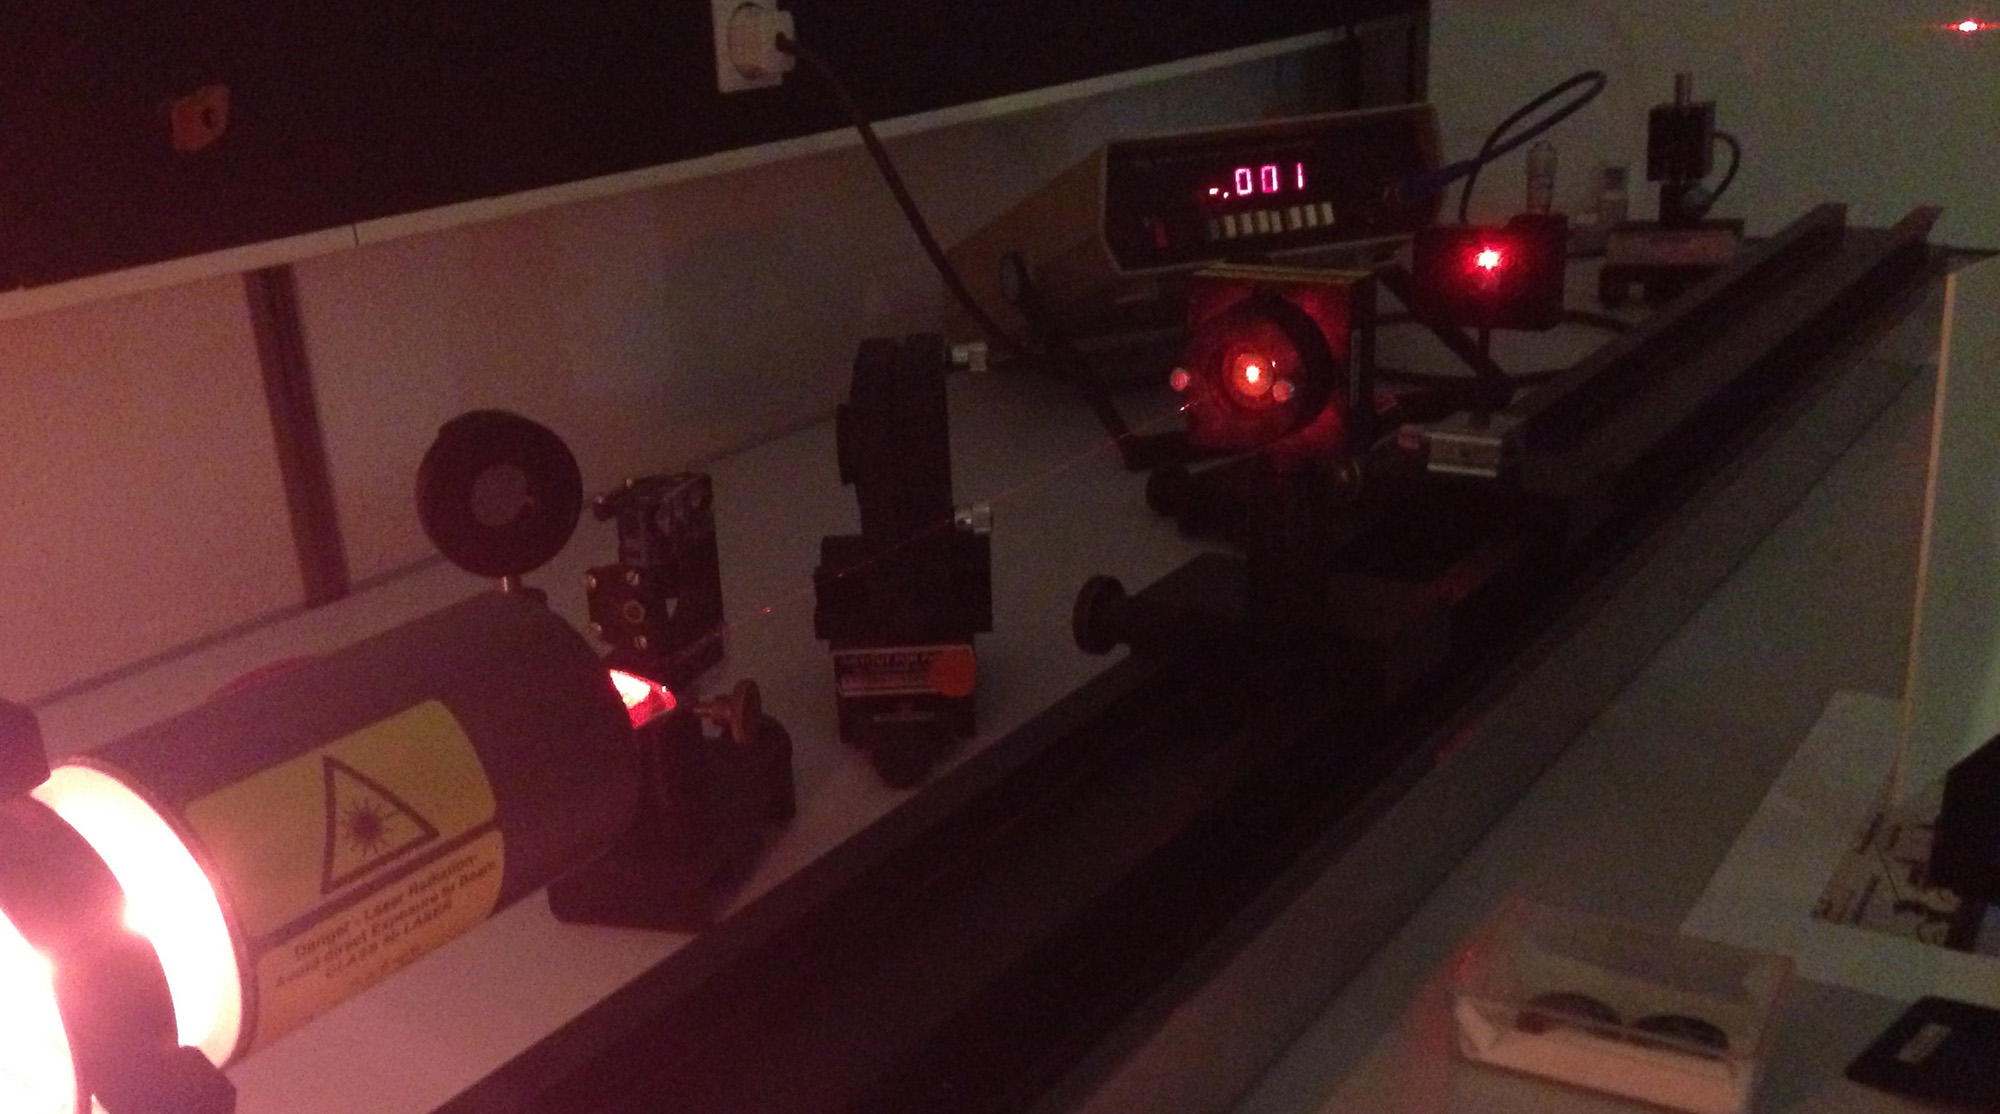
\includegraphics[width=0.9\linewidth]{img/laser.jpg}
    \caption{Funktionierender HeNe-Laser.}
    \label{fig:laser}
\end{figure}
